\section{Introduction}
\subsection{OpenPGP}
\begin{frame}
    \frametitle{\color{white}OpenPGP}
    \begin{block}{Qu'est ce que OpenPGP ?}
    	\begin{itemize}
         \item Standard cryptographique normalisé dans la RFC 4880.
         \item Décrit des formats de messages adaptés aux outils permettant l’envoi ou le stockage sécurisé.
         \item Repose sur un système hybride de cryptographie (symétrique + asymétrique).
       \end{itemize} 
    \end{block}
\end{frame}

\subsection{GnuPG}
\begin{frame}
    \frametitle{\color{white}GnuPG}
    \begin{block}{Qu'est ce que GnuPG ?}
      \begin{itemize}
        \item GnuPG (GNU Privacy Guard) est une implantation libre d'OpenPGP.
        \item Basé sur le logiciel PGP.
        \item Permet la gestion d'un trousseau de clefs asymétriques.
        \item Propose un modèle de toile de confiance.
        \item Permet le chiffrement/déchiffrement, la signature/vérification, la certification et l'authentification.
      \end{itemize}
    \end{block}
\end{frame}

\subsection{Le besoin}
\begin{frame}
    \frametitle{\color{white}Le besoin}
    \begin{block}{Quels besoin ?}
    	\begin{itemize}
         \item Une étude détaillée d'OpenPGP et de GnuPG.
         \item Une interface graphique permettant de facilité la compréhension et l'utilisation de GnuPG.
         \item Une étude des limites, et une implantation d'une attaque sur les identifiants de clefs PGP.
       \end{itemize} 
    \end{block}
\end{frame}

\subsection{Équipe}
\begin{frame}
    \frametitle{\color{white}Équipe}
  \begin{center}
    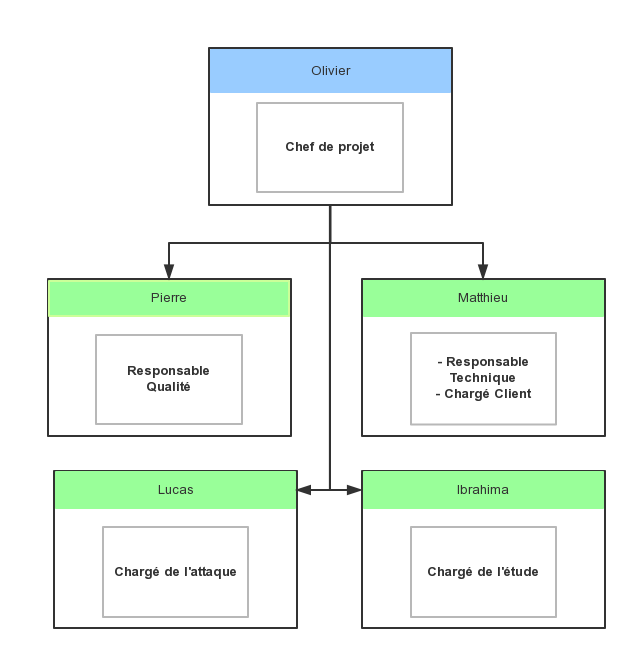
\includegraphics[scale=0.30]{guipgteam.png}
  \end{center}
\end{frame}
